\documentclass[
]{scrartcl}

%Deutsche Sprachunterstützung
\usepackage[utf8]{inputenc}
\usepackage[ngerman]{babel}
\usepackage{marvosym}
\DeclareUnicodeCharacter{20AC}{\EUR}

%Für das Einbinden von Bildern
\usepackage{graphicx}

%Tabellen
\usepackage{array}

%Tabellen automatisch schoener
\usepackage{booktabs}

%Caption
\usepackage{caption}
\usepackage{subcaption}

%Formeln
\usepackage{mathtools}
\usepackage{amsmath}
\usepackage{amssymb}
\usepackage{amstext}
\usepackage{dsfont}

%\usepackage{mnsymbol}

%Vectorpfeile schöner
\usepackage{esvect}

%Formatierung
\usepackage[T1]{fontenc}
\usepackage{lmodern}
\usepackage{microtype}

%Schaltbilder malen
\usepackage[europeanresistors,cuteinductors,siunitx]{circuitikz}

%\usepackage[german=guillemets]{csquotes}

%Formatierungsanweisungen
\newcommand{\wichtig}[1]{\underline{\large{#1}}}
\newcommand{\aref}[1]{(s.Abb. \ref{#1})}
\newcommand{\R}{\mathbb{R}}
\newcommand{\K}{\mathbb{K}}
\newcommand{\C}{\mathbb{C}}
\begin{document}

\title{Frequenzfilter}
\subtitle{1. Versuch PPG 8}
\date
%\author{PPG8}
\maketitle
\section{Vorwort}
blabla bulbbaslkdfalskdf

\section{Theoretische Betrachtung}
\subsection{Durchlassfilter}
Ein Durchlassfilter ist eine Reihenschaltung aus Kondensator, Spule und Widerstand. Sieh Abbildung \ref{plan:durchlass} auf Seite \pageref{plan:durchlass}.\\
Mit den Kirchhoffschen Regeln und 
$
U=Z\cdot I
$ 
gilt:
\begin{equation}
U_a=\frac{R}{R+i\left(\omega L-\frac{1}{\omega C}\right)}\cdot U_e\\
\end{equation}
\begin{equation}
\Rightarrow\left| U_a \right| = \frac{R}{\sqrt{R^2+\left(\omega L - \frac{1}{\omega C}\right)}}\cdot \left| U_e \right|
\end{equation}
Bei der Frequenz
\begin{equation}
\omega=\omega_R=\frac{1}{\sqrt{L\cdot C}}
\end{equation}
wird
$
\left|U_a \right| = \left|U_e \right|
$
, d.h. die Wechselspannung $U_e(\omega_R)$ wird vollständig durchgelassen, während alle anderen Frequenzen abgeschwächt werden.
  Setzt man nun
\begin{equation}
\frac{\left|U_a \right|}{\left|U_e \right|}=\frac{1}{\sqrt{2}}
\end{equation}
und löst die quadratische Gleichung, ergibt sich die Bedingung
\begin{equation}
\omega_{1,2}=\pm \frac{R}{2L}+\sqrt{\frac{R^2}{4L^2}+\omega_R^2}
\end{equation}
Berechnet man nun die Frequenzbreite
$
\Delta \omega=\omega_1-\omega_2
$
, ergibt sich
\begin{equation}
\Delta \omega=\frac{R}{L}
\end{equation}
, d.h. bei kleineren Widerständen ergeben sich 'schärfere' Peaks.
\\
Diese Betrachtung nimmt an, dass der Ohmsche Widerstand der Spule vernachlässigbar ist, was in der Praxis jedoch nicht immer der Fall ist.
Wenn die Spule einen Widerstand $R_L$ besitzt, ändert sich Gleichung (2) zu
\begin{equation}
\Rightarrow\left| U_a \right| = \frac{R}{\sqrt{(R+R_L)^2+\left(\omega L - \frac{1}{\omega C}\right)}}\cdot \left| U_e \right|
\end{equation}
also wird die Wechselspannung $U_e$ selbst bei der Resonanzfrequenz nicht vollständig durchgelassen.
\begin{figure}
\centering
\begin{circuitikz}[european voltages]
\draw
  (0,0) to [short, -o] (6,0)
  (6,0) to [open, l_=$U_a$] (6,4) %Ausgangsspannung
  %to [voltmeter, l_=$U_a$] (6,4) % Messung
  (6,4) to [short, o-] (5,4) 

  (0,0) to [csV, l=$U_e$] (0,4) % Eingangsspannung
  to [short] (1,4)
  to [C, l=$C$] (3,4) % Kondensator
  to [L, l=$L$] (5,4) % Spule
  to [R, l_=$R_m$] (5,0); % Messwiderstand

\end{circuitikz}
\caption{Schaltbild Durchlassfilter}
\label{plan:durchlass}
\end{figure}
\subsection{Sperrfilter}
Beim Sperrfilter werden die Spule und der Kondensator nun parallel geschaltet. (hier Schaltbild einfügen)
Analog zum Durchlassfilter ergibt sich nun
\begin{equation}
U_a=\frac{R}{R-i \frac{1}{\omega C - \frac{1}{\omega L}}}\cdot U_e\\
\end{equation}
\begin{equation}
\Rightarrow\left| U_a \right| = \frac{R}{\sqrt{R^2+\frac{1}{(\omega C - \frac{1}{\omega L})^2}}}\cdot \left| U_e \right|
\end{equation}
Bei der Resonanzfrequenz (3) geht nun $\left| U_a \right|\longrightarrow 0$, d.h. die Frequenz $\omega_R$ wird blockiert, während andere Frequenzen durchgelassen werden.
\footnotesize
\begin{align}
&\left| \frac{U_a}{U_e} \right| =  \\
&\frac{R\left(R^2_L+\omega ^2\left[C\left(R^2_L+\omega ^2 L^2 \right) - L\right] ^2 \right)}{\sqrt{ \left( R^2_L + \omega ^2L^2\right) R_L+R_{ges}\left\{ R_L^2+\omega ^2\left[ C\left( R_L^2+\omega ^2L^2\right) -L\right] ^2\right\}^2+\left(R^2_L+\omega^2L^2\right)^2\omega^2\left[C\left(R^2_L+\omega^2L^2\right)-L\right]}}\nonumber
\end{align}
\normalsize
\begin{figure}
\centering
\begin{circuitikz}
\draw
  (0,1) to [short, -o] (6,1)
  (6,1) to [open, l_=$U_a$] (6,4) %Ausgangsspannung
  (6,4) to [short, o-] (5,4) 

  (0,1) to [csV, l=$U_e$] (0,4) % Eingangsspannung
  to [short, ] (1,4)
  (1,5) to [short] (1,3)
  to [C, l_=$C$] (4,3) % Kondensator
  to [short] (4,5)
  to [L, l=$L$] (1,5) % Spule
  (4,4) to [short] (5,4) 
  to [R, l_=$R_m$] (5,1); % Messwiderstand
\end{circuitikz}
\caption{Schaltbild eines Sperrfilters}
\label{plan:sperr}
\end{figure}
\section{Versuchsdurchführung}
Nach einigen Messversuchen


Der Schaltkreis hat 2,7 Ohm + dem Messwiderstand.





\begin{figure}[t]
\centering
	\subcaptionbox{Durchlassfilter\label{img:durchlass}}[.4\linewidth]
		{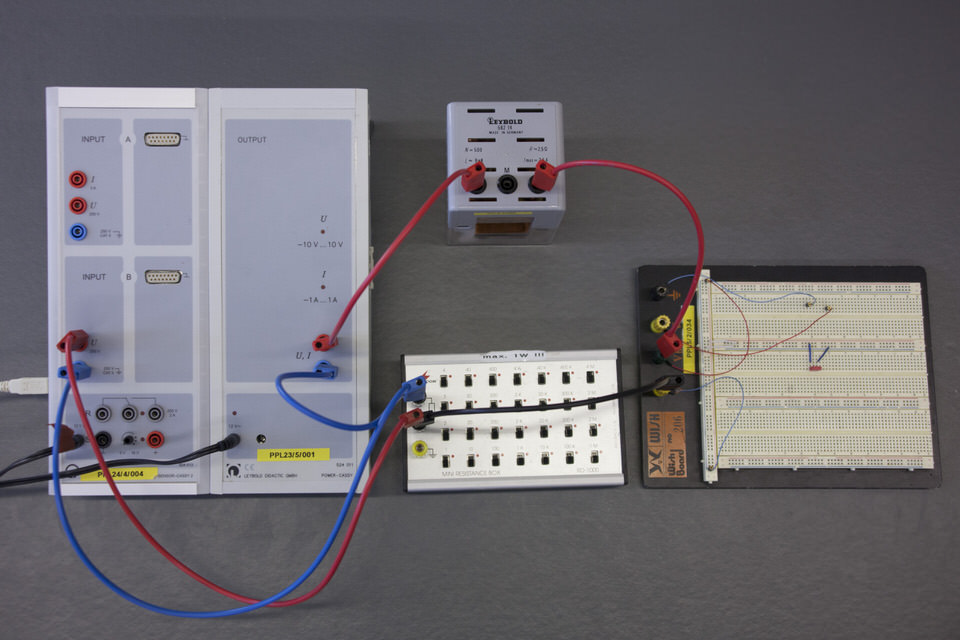
\includegraphics[width=.4\textwidth]{images/durchlassfilter}}
	\subcaptionbox{Sperrfilter\label{img:sperr}}[.4\linewidth]
		{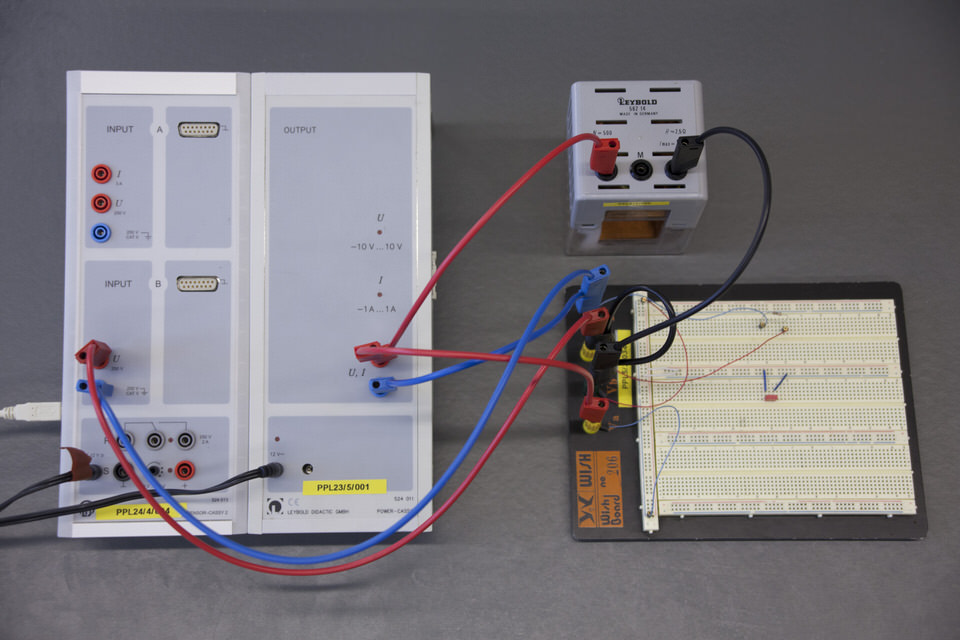
\includegraphics[width=.4\textwidth]{images/sperrfilter}}
\caption{Fotos der Versuchsaufbauten}
\end{figure}
\section{Versuchsdurchführung}
Nach einigen Messversuchen


Der Schaltkreis hat 2,7 Ohm + dem Messwiderstand.
\section{Diskussion der Ergebnisse}






\end{document}